\section{Rezolvarea numerică a ecuațiilor algebrice prin metoda tangentei.}

\textbf{Metoda tangentei} (metoda lui Newton) este una din cele mai eficiente metode 
iterative de rezolvare a ecuațiilor neliniare. \par

Fie o ecuație de forma $f(x)=0$, cu variabile $x \in [a,b]$, pentru care s-a 
separat în prealabil o soluție în intervalul $[a,b]$ (folosind metoda 
bisecției, spre exemplu), adică $f(a) \cdot f(b) <0$. \par

\begin{figure}[H]
    \centering
    \includestandalone{assets/tangent-plot}
    \caption{Demonstrarea grafică a metodei tangentei.}
    \label{fig:tangent-figure}
\end{figure}

\textit{Metoda lui Newton} poate fi interpretată geometric ca o trasare repetată a 
tangentelor la funcție, prin punctele de aproximare a soluției, până când 
tantenta intersectează punctul în care funcția se anulează, ori un punct 
delimitat cu o anumită precizie de soluția exactă.

\begin{figure}[H]
    \centering
    \includestandalone[scale=0.7]{assets/tangent-flowchart}
    \caption{Diagrama metodei tangentei.}
    \label{fig:tangent-flowchart}
\end{figure}

\lstinputlisting[language={[Sharp]C}]{assets/listings/Newton.cs} \par

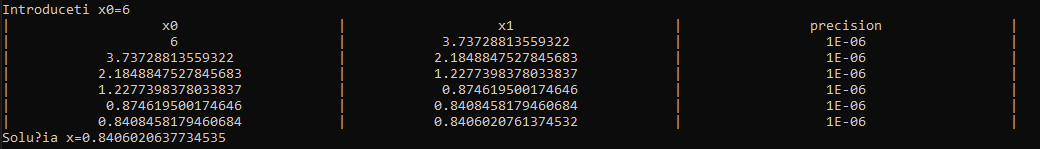
\includegraphics[width=0.8\textwidth]{assets/listings/newton-output.png} \par

\clearpage
